\documentclass{article}
\usepackage{listings}
\usepackage[a4paper, total={6in, 8in}]{geometry}
\usepackage{graphicx}

\title{CMOR 421/521, Homework \#1: \LaTeX{} Submission}
\author{\texttt{amc50}}
\date{February 29, 2024}

\begin{document}
\maketitle

\section{Compilation}

\subsection{Accessing NOTS Cluster}
\begin{verbatim}
It is important to note that the following process is done on Rice Owls Network. 
If this is not the case, this would be unsuccessful. 

Command used to ssh into NOTS:
MacBook-Pro-95:cmor-421-521-submissions antoniocrivello$ ssh amc50@nots.rice.edu

Command used to activate interactive node on NOTS:
[amc50@nlogin1 ~]$ 
srun --pty --partition=interactive --ntasks=1 --mem=1G --time=00:30:00 $SHELL

Command used to load modules needed for compilation:
[amc50@bc9u7n1 ~]$ module load GCC/13.1.0         

To access files created on local desktop, a GitHub Repository is used. As such, 
this repository must be cloned on the cluster. This process requires a password-protected key.

Command used to generate SSH key :
[amc50@bc9u7n1 ~]$ ssh-keygen -t ed25519 -C "amc50@rice.edu"

Command used to access public key:
[amc50@bc9u7n1 ~]$ emacs ~/.ssh/id_ed25519.pub 

After accessing the SSH key, it is added to the GitHub The key was then added 
to list of SSH keys on GitHub.

Command used to clone cmor-421-521-submission GitHub repository:
[amc50@bc9u7n1 ~]$ 
git clone git@github.com:AntonioCrivello/cmor-421-521-submissions.git

For compilation on the NOTS Cluster I am utilizing a Makefile. 

Set of commands to compile project: 
[amc50@bc9u7n1 homework-1]$ make clean
Output of make clean:
rm -f matmul_recursive ./obj/*.o *~ *.o

[amc50@bc9u7n1 homework-1]$ make
Output of make:
g++ -c src/matrix.cpp -o obj/matrix.o -I./include -O3 -std=c++11
g++ obj/matrix.o main.cpp -I./include -O3 -std=c++11 -o matmul_recursive

In order to efficiently generate timings for matrix sizes of 2^i for 
i = 4,5,6 ... 10, I have created a bash script to run the aforementioned 
make clean and make commands with the matrix size as an argument. Additionally,
at the initial phase of the project to determine the optimal block size for
each matrix-matrix multiplication the block size is also supplied as an argument
to the executable.

Command used to generate timings and compile project:
[amc50@bc9u7n1 homework-1]$ ./generate-timings.sh 
\end{verbatim}

\section{Matrix-Matrix Multiplication}

\subsection{Column Major Storage for Matrix-Matrix Multiplication}
\begin{verbatim}
If the matrix was stored in column major format instead of row major format for
matrix-matrix multiplication a few changes should be made. The first is to change how
the memory is accessed during the impementation. With row major storage the memory is 
efficiently access by looping through the rows and then the columns. For the column 
major formatting, this should be changed, looping through the column first and then the
row. This will allow the required data values to be located adjacent to each other. There
is also a benefit in unrolling the innermost loop to reduce overhead and utilize the
location of the column values.
\end{verbatim}

\subsection{Matrix Transpose}
\begin{lstlisting}[mathescape=true]
For matrices stored in column major format it is expected that $A^TB$ would be faster 
than AB. The primary reason this is the case is because when applying the transpose 
to matrix A and then multiplying to matrix B, the matrix-matrix multiplication involves 
looping through the rows of $A^T and the columns of B. Given then that A is stored in 
column major format, the transpose of the columns is the rows so the memory accessing 
will be contiguous. This is an improvement over the noncontiguous accessing that is 
required for row major containing. 
\end{lstlisting}



\section{Optimizing Matrix-Matrix Multiplication}

\subsection{Timing}
\begin{table}[ht!]
    \caption{Naive Matrix-Matrix Multiplication Timings on NOTS}
    \centering
    \begin{tabular}{|c|c|c|c|c|c|c|c|c|c|}
        \hline
        Matrix Size & n = 4 & n = 8 & n = 16 & n = 32 & n = 64 & n = 128 & n = 256 & n = 512 & n = 1024 \\
        \hline
        n = 16 & 2.9041e-05 & 3.3614e-05 & 3.2159e-05 \\
        \hline
        n = 32 & 0.000222842 & 0.00025741 & 0.000259517 & 0.00028529 \\
        \hline
        n = 64 & 0.00205113 & 0.00200312 & 0.00167115 & 0.00158465 & 0.00150467 \\
        \hline
        n = 128 & 0.0120923 & 0.0121557 & 0.0115599 & 0.0111493 & 0.0119782 & 0.014615 \\
        \hline
        n = 256 & 0.158795 & 0.131669 & 0.140042 & 0.137167 & 0.134298 & 0.153463 & 0.149298 \\
        \hline
        n = 512 & 1.27346 & 1.14611 & 1.0844 & 1.07697 & 1.23491 & 1.19583 & 1.15814 & 1.05354 \\
        \hline 
        n = 1024 & 11.4279 & 14.3977 & 12.306 & 11.8852 & 10.7746 & 12.3554 & 12.6266 & 14.937 \\
        \hline
    \end{tabular}
\end{table}

\begin{table}[ht!]
    \caption{Blocked Matrix-Matrix Multiplication Timings on NOTS}
    \centering
    \begin{tabular}{|c|c|c|c|c|c|c|c|c|c|}
        \hline
        Matrix Size & n = 4 & n = 8 & n = 16 & n = 32 & n = 64 & n = 128 & n = 256 & n = 512 & n = 1024 \\
        \hline
        n = 16 & 2.3312e-05 & 2.0671e-05 & 1.8851e-05 \\
        \hline
        n = 32 & 0.000196252 & 0.000195223 & 0.000194868 & 0.000180096 \\
        \hline
        n = 64 & 0.00178605 & 0.00150001 & 0.0011403 & 0.00112655 & 0.00115903 \\
        \hline
        n = 128 & 0.0105116 & 0.00939145 & 0.00799496 & 0.00823802 & 0.00810977 & 0.0105357 \\
        \hline
        n = 256 & 0.102929 & 0.0823619 & 0.0791603 & 0.0769003 & 0.0808152 & 0.0836151 & 0.0974383 \\
        \hline
        n = 512 & 0.753265 & 0.621876 & 0.580653 & 0.555099 & 0.679861 & 0.751526 & 0.77674 & 0.777467 \\
        \hline 
        n = 1024 & 6.20977 & 5.36031 & 4.86852 & 4.55242 & 6.04679 & 6.17169 & 6.34725 & 6.25861 \\
        \hline
    \end{tabular}
\end{table}

\subsection{Discussion}

\begin{verbatim}

Does this depend on the size of the matrix?
    
\end{verbatim}

\subsection{Roofline Plot Results}
\begin{figure}[!htb]
    \centering
    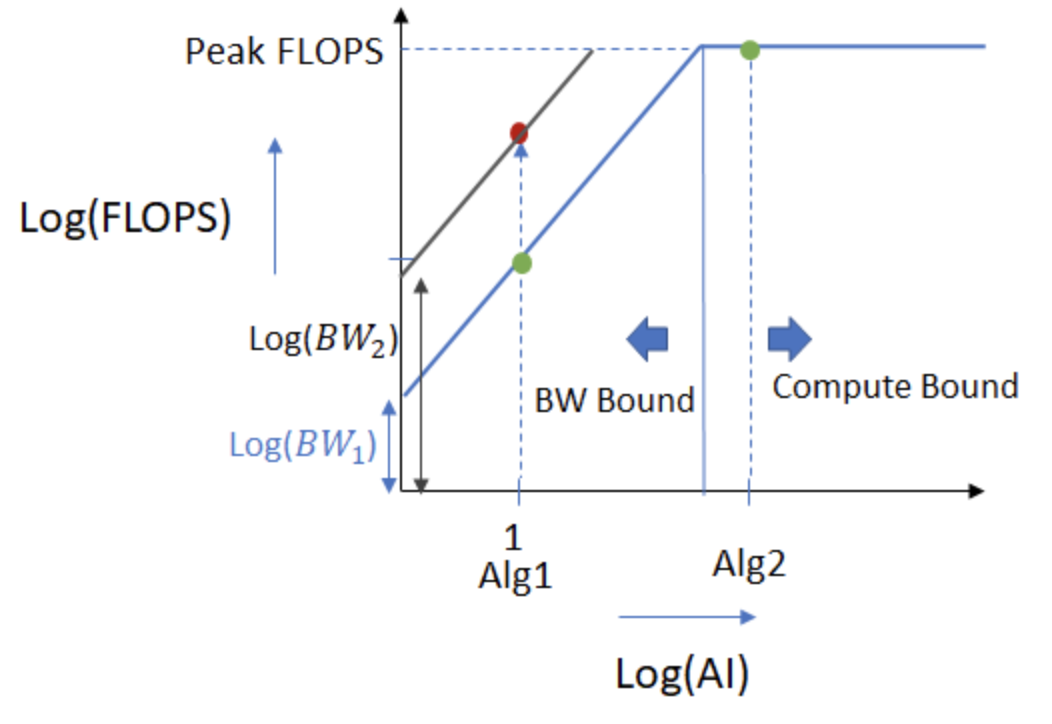
\includegraphics[width=0.8\linewidth]{roofline_plot.png}
    \caption{Roofline Plot for Naive Matrix-Matrix Multiplication}
\end{figure}

\begin{figure}[!htb]
    \centering
    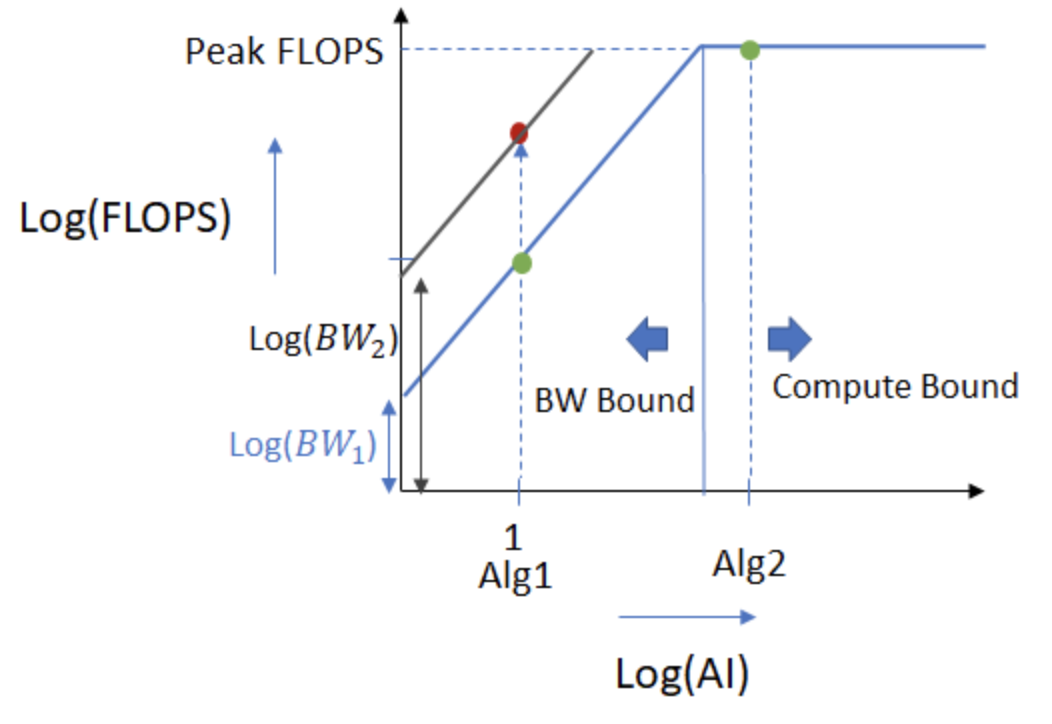
\includegraphics[width=0.8\linewidth]{roofline_plot.png}
    \caption{Roofline Plot for Blocked Matrix-Matrix Multiplication}
\end{figure}


\section{Recursive Matrix-Matrix Multiplication}

\subsection{Timing}

\begin{table}[ht!]
    \caption{Blocked Matrix-Matrix Multiplication Timings on NOTS}
    \centering
    \begin{tabular}{|c|c|c|c|c|c|c|c|c|c|}
        \hline
        Matrix Size & n = 4 & n = 8 & n = 16 & n = 32 & n = 64 & n = 128 & n = 256 & n = 512 & n = 1024 \\
        \hline
        n = 16 & 2.3312e-05 & 2.0671e-05 & 1.8851e-05 \\
        \hline
        n = 32 & 0.000196252 & 0.000195223 & 0.000194868 & 0.000180096 \\
        \hline
        n = 64 & 0.00178605 & 0.00150001 & 0.0011403 & 0.00112655 & 0.00115903 \\
        \hline
        n = 128 & 0.0105116 & 0.00939145 & 0.00799496 & 0.00823802 & 0.00810977 & 0.0105357 \\
        \hline
        n = 256 & 0.102929 & 0.0823619 & 0.0791603 & 0.0769003 & 0.0808152 & 0.0836151 & 0.0974383 \\
        \hline
        n = 512 & 0.753265 & 0.621876 & 0.580653 & 0.555099 & 0.679861 & 0.751526 & 0.77674 & 0.777467 \\
        \hline 
        n = 1024 & 6.20977 & 5.36031 & 4.86852 & 4.55242 & 6.04679 & 6.17169 & 6.34725 & 6.25861 \\
        \hline
    \end{tabular}
\end{table}

\subsection{Implementation Analysis}
\begin{verbatim}

Determine Optimal Block Size

How to check correct implementation

\end{verbatim}

\subsection{Results}
\begin{figure}[!htb]
    \centering
    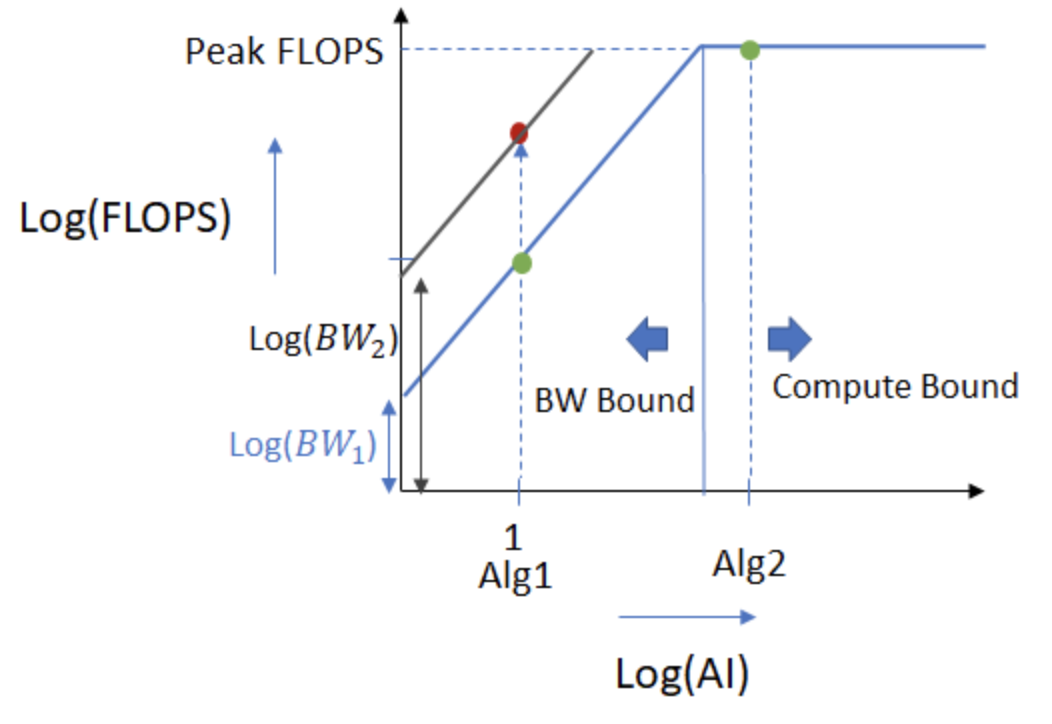
\includegraphics[width=0.8\linewidth]{roofline_plot.png}
    \caption{Roofline Plot for Recursive Matrix-Matrix Multiplication}
\end{figure}

\subsection{Discussion}

\begin{verbatim}

    Timing Comparison

    1.1. not much improvement
    1.2.Column column. when transpose row column

    2.1. does not depend on matrix size. it depends on cache size. unless block size is smaller than matrix
    2.2. slide 4 is helpful for roofline

    3.1.2 what is a microkernel
    3.2. & in recursion?

    Questions:
    - How to do roofline plot
    - Why is distributed not faster
    - What is a microkernel
    - Why only one & in recursion
    - Pass a copy of C?
    - How to check?

\end{verbatim}

\begin{comment}
    Generating public/private ed25519 key pair.
    Enter file in which to save the key (/home/amc50/.ssh/id_ed25519): 
    Enter passphrase (empty for no passphrase): 
    Enter same passphrase again: 
    Your identification has been saved in /home/amc50/.ssh/id_ed25519.
    Your public key has been saved in /home/amc50/.ssh/id_ed25519.pub.
    The key fingerprint is:
    SHA256:1Xu4gV32DaSy0mP1qHGao7fMWMgxI6UWWx7PYAILwSY amc50@rice.edu
    The key's randomart image is:
    +--[ED25519 256]--+
    | .o..         .  |
    |E o. o     . o   |
    | o  . o * o + +  |
    |       X B * B o.|
    |      = S X B o o|
    |     . o B B +   |
    |        o * .    |
    |         *..     |
    |        o.+.     |
    +----[SHA256]-----+
    \end{comment}

    \begin{comment}
        Cloning into 'cmor-421-521-submissions'...
        Warning: Permanently added the ECDSA host key for IP address '140.82.114.3' 
        to the list of known hosts.
        \end{comment}

    
    %Intel(R) Xeon(R) CPU E5-2650 v2 @ 2.60GHz: GFLOPS: 166.4 APP: 0.04992
    %https://www.intel.com/content/dam/support/us/en/documents/processors/APP-for-Intel-Xeon-Processors.pdf
    %Dividing by number of cores

    %20.8

    % n = 512
    % b = 8

    %Blocked: CI = 2n^3 / (2n^2 + 2 * n^3 / b)
    %Runtime: .103s
    %peak_bandwidth = 59.7, GB / S
    %peak_performance = 166.4 / 8

    %GFLOPS_per_sec = (2 * n ^ 3 / 1e9) / runtime
    %(2 * n ^ 3 / 1e9) = GFLOPS

    %CI = Flops / byte = 2n^3 / [(2n^2 + 2n^3/b) * (# bytes = 8)]
    
    %Naive: CI = 2n^3 / 3n^2 + n^3 ~ 2 / 8
    %Recursive: CI = 2n^3 / 
    %Recursive: CI ~ b
    %Recursive: CI = 2/3 * b


    %roofline = min(peak_performance, CI * peak_bandwidth)

\end{document}
